\chapter{Functions}
A C function is somewhat similar to an assembly subroutine in that it is a block of code which can be called and which returns back to where it was called from on completion. As the name implies, functions are typically coded to provide some defined, useful functionality. 

A difference between C functions and assembly subroutines is that functions have a defined interface which allows the passing of data into them in the form of arguments as well as the returning of data. There can be zero or one elements returned from a function. There can be 0 or many arguments passed to a function.

In essence, a function can be though of as some block of processing which optionally takes in data and optionally returns data. This is shown graphically in \autoref{fig:function}.

\begin{figure}
\centering
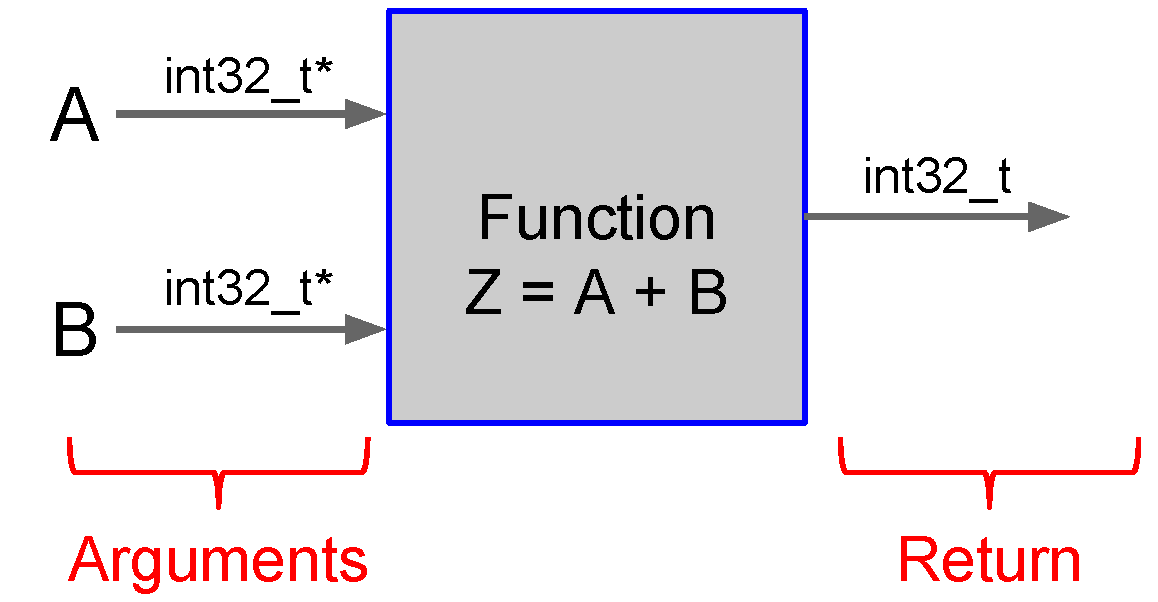
\includegraphics[scale=0.5]{./week9/function.pdf}
\caption{Function}
\label{fig:function}
\end{figure}

The general form for a function is shown below.

\begin{lstlisting}[language=c]
returnType  functionName(type parameter0, type parameter1, ...) {
    // code to implement function
}
\end{lstlisting}

With this in mind, a possible implementation for the block diagram shown in \autoref{fig:function} would be as follows. 

\begin{lstlisting}[language=c]
int32_t pointer_adder(int32_t *a_ptr, int32_t *b_ptr) {
    int32_t sum;
    sum = *a_ptr + *b_ptr;
    return sum;
}
\end{lstlisting}

\section{Function Prototypes}
Whenever a line of code calls a function, that line of code should 'know' what the function it is calling looks like in terms of parameters and return type. 
This is to ensure that the compiler can warn you if you attempt to use the function incorrectly by (for example) supplying a pointer as an argument when the function expects a basic number.
In order for the calling line to know what the function looks like, the function should be \emph{declared} before it is called.
There is a difference between declaring a function and defining a function. 
Declaring simply shows what the function is called, what it return as what it takes.
Defining provides the declaration as well as the code which implements the function. 
The code for the \texttt{pointer\_adder} which we saw above was a function definition. A function declaration for \texttt{pointer\_adder} would look as follows\footnote{You are able to supply names as well as type in the function parameter list, but they are not necessary and don't really do anything for a declaration}.

\begin{lstlisting}[language=c]
int32_t pointer_adder(int32_t, int32_t);
\end{lstlisting}

Notice how that declaration shows the `black box' appearance of the function and not what the function actually does.
Typically we write all of our function declarations (or prototypes) at the start of the source file and then the definitions (or implementations) after that. 
That way any time a function is called, the declaration will have already been seen by the compiler so the compiler will be able to check that the way you are using the function matches the structure of the function.

